\section{Testplan}

\subsection{Einführung}

Der Testplan beschreibt alle wichtigen Testfälle und ihre erwarteten Resultate.

\subsubsection{Ablaufplan}
\begin{figure}
	\centering
	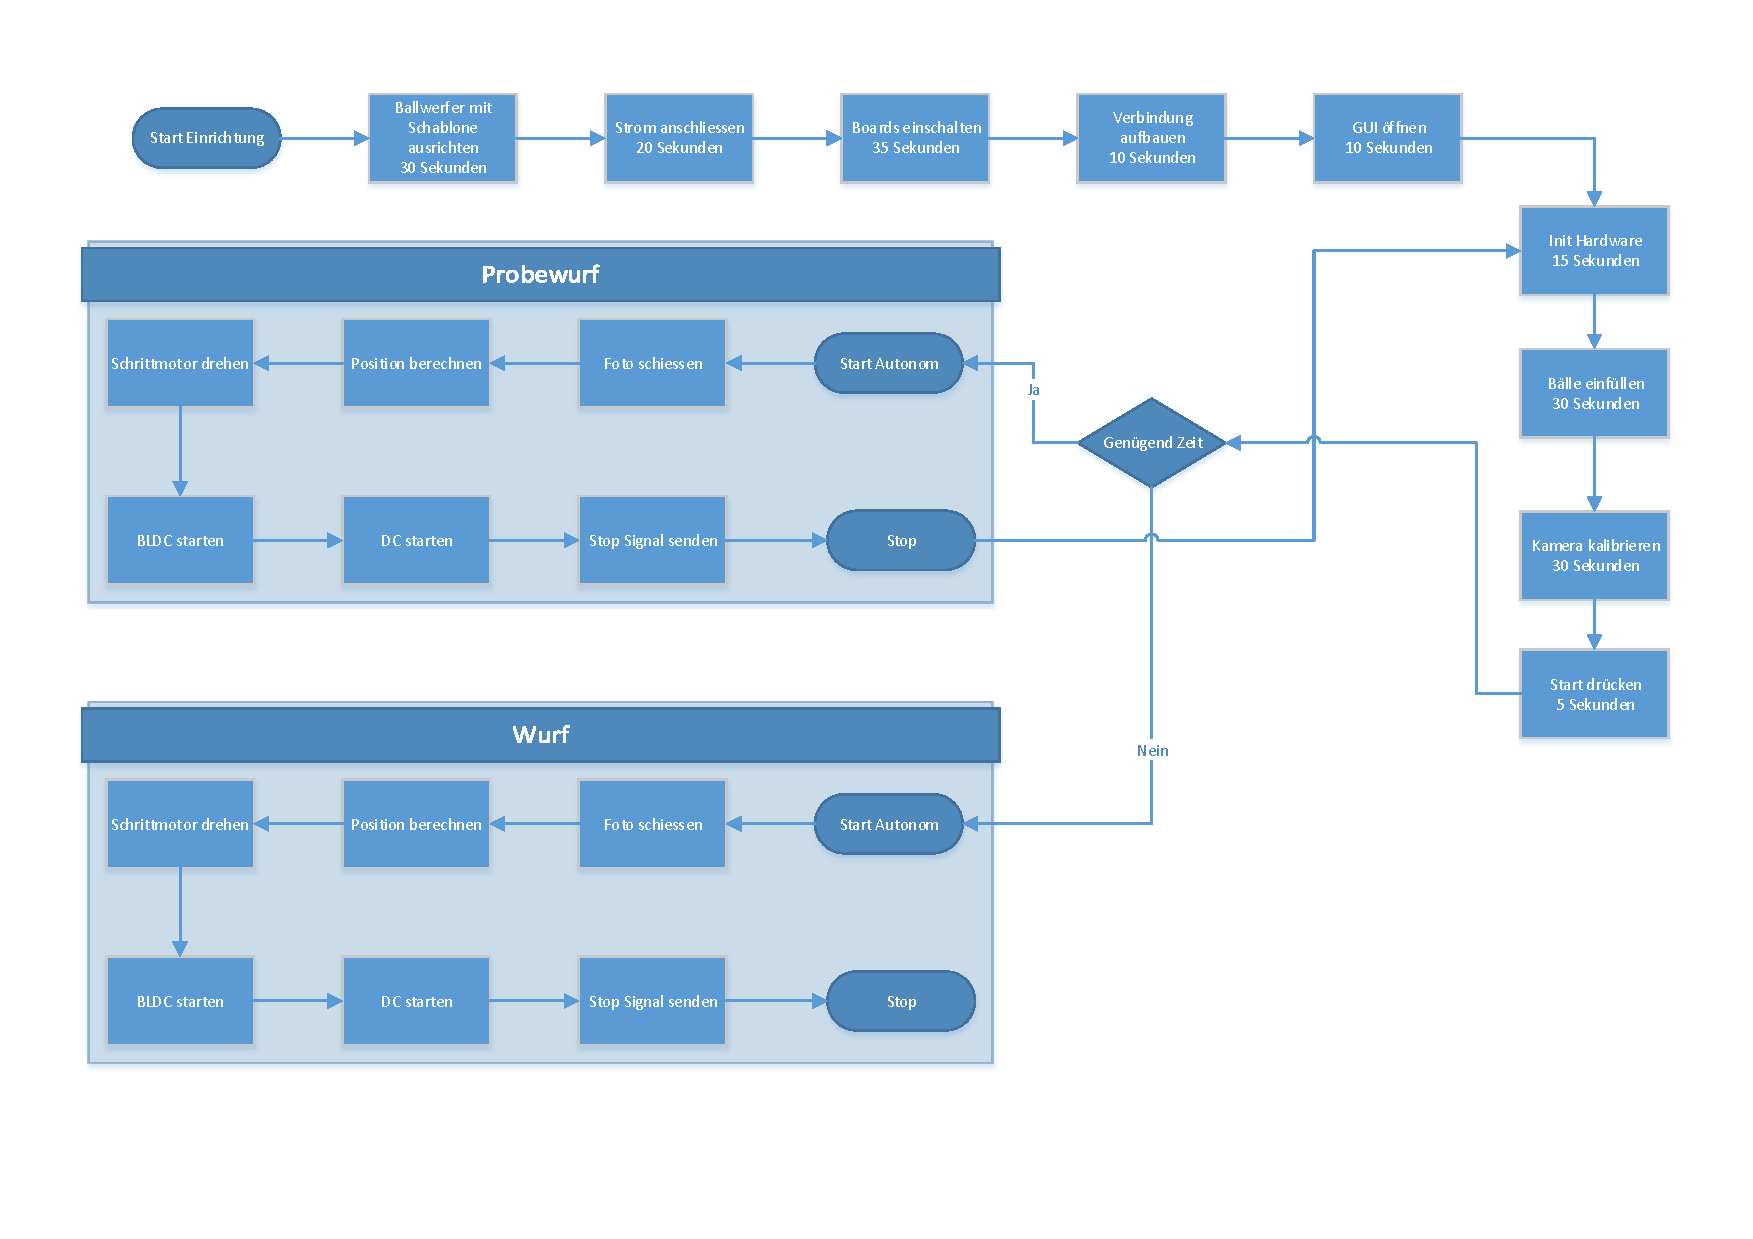
\includegraphics[width=0.9\linewidth]{../../fig/ablauf-ballwurf}
	\caption{}
	\label{fig:ablauf-ballwurf}
\end{figure}

\subsection{Gesamtsystemtest}

\subsubsection{Ballwerfer ausgerichtet}
\begin{table}[h!]
	\renewcommand{\arraystretch}{1.5}
	\begin{tabular}{|r|p{14cm}|}
		\hline Beschreibung & Der DC Motor lässt sich via GUI ansteuern. \\ 
		\hline Vorbedingungen & SYS102 \\ 
		\hline Testdaten & Konfigurationsdaten \\ 
		\hline Vorgehen & 
		\begin{enumerate}
			\item Configurator starten
			\item Schritte anpassen
			\item Motor starten
			\item Motor stoppen
			\item Motor reset
		\end{enumerate} \\ 
		\hline Ergebnis & Der Motor wird sich um die entsprechende Anzahl Schritte drehen. Zusätzlich nimmt er seine Ausgangsposition beim Reset an. \\ 
		\hline 
	\end{tabular}
\end{table}

\subsubsection{Strom angeschlossen}
\begin{table}[h!]
	\renewcommand{\arraystretch}{1.5}
	\begin{tabular}{|r|p{14cm}|}
		\hline Beschreibung & Der DC Motor lässt sich via GUI ansteuern. \\ 
		\hline Vorbedingungen & SYS102 \\ 
		\hline Testdaten & Konfigurationsdaten \\ 
		\hline Vorgehen & 
		\begin{enumerate}
			\item Configurator starten
			\item Schritte anpassen
			\item Motor starten
			\item Motor stoppen
			\item Motor reset
		\end{enumerate} \\ 
		\hline Ergebnis & Der Motor wird sich um die entsprechende Anzahl Schritte drehen. Zusätzlich nimmt er seine Ausgangsposition beim Reset an. \\ 
		\hline 
	\end{tabular}
\end{table}

\subsubsection{Boards eingeschaltet}
\begin{table}[h!]
	\renewcommand{\arraystretch}{1.5}
	\begin{tabular}{|r|p{14cm}|}
		\hline Beschreibung & Der DC Motor lässt sich via GUI ansteuern. \\ 
		\hline Vorbedingungen & SYS102 \\ 
		\hline Testdaten & Konfigurationsdaten \\ 
		\hline Vorgehen & 
		\begin{enumerate}
			\item Configurator starten
			\item Schritte anpassen
			\item Motor starten
			\item Motor stoppen
			\item Motor reset
		\end{enumerate} \\ 
		\hline Ergebnis & Der Motor wird sich um die entsprechende Anzahl Schritte drehen. Zusätzlich nimmt er seine Ausgangsposition beim Reset an. \\ 
		\hline 
	\end{tabular}
\end{table}

\subsubsection{Verbindung aufgebaut}
\begin{table}[h!]
	\renewcommand{\arraystretch}{1.5}
	\begin{tabular}{|r|p{14cm}|}
		\hline Beschreibung & Der DC Motor lässt sich via GUI ansteuern. \\ 
		\hline Vorbedingungen & SYS102 \\ 
		\hline Testdaten & Konfigurationsdaten \\ 
		\hline Vorgehen & 
		\begin{enumerate}
			\item Configurator starten
			\item Schritte anpassen
			\item Motor starten
			\item Motor stoppen
			\item Motor reset
		\end{enumerate} \\ 
		\hline Ergebnis & Der Motor wird sich um die entsprechende Anzahl Schritte drehen. Zusätzlich nimmt er seine Ausgangsposition beim Reset an. \\ 
		\hline 
	\end{tabular}
\end{table}

\subsubsection{GUI geöffnet}
\begin{table}[h!]
	\renewcommand{\arraystretch}{1.5}
	\begin{tabular}{|r|p{14cm}|}
		\hline Beschreibung & Der DC Motor lässt sich via GUI ansteuern. \\ 
		\hline Vorbedingungen & SYS102 \\ 
		\hline Testdaten & Konfigurationsdaten \\ 
		\hline Vorgehen & 
		\begin{enumerate}
			\item Configurator starten
			\item Schritte anpassen
			\item Motor starten
			\item Motor stoppen
			\item Motor reset
		\end{enumerate} \\ 
		\hline Ergebnis & Der Motor wird sich um die entsprechende Anzahl Schritte drehen. Zusätzlich nimmt er seine Ausgangsposition beim Reset an. \\ 
		\hline 
	\end{tabular}
\end{table}

\subsubsection{Reset Motoren}
\begin{table}[h!]
	\renewcommand{\arraystretch}{1.5}
	\begin{tabular}{|r|p{14cm}|}
		\hline Beschreibung & Der DC Motor lässt sich via GUI ansteuern. \\ 
		\hline Vorbedingungen & SYS102 \\ 
		\hline Testdaten & Konfigurationsdaten \\ 
		\hline Vorgehen & 
		\begin{enumerate}
			\item Configurator starten
			\item Schritte anpassen
			\item Motor starten
			\item Motor stoppen
			\item Motor reset
		\end{enumerate} \\ 
		\hline Ergebnis & Der Motor wird sich um die entsprechende Anzahl Schritte drehen. Zusätzlich nimmt er seine Ausgangsposition beim Reset an. \\ 
		\hline 
	\end{tabular}
\end{table}

\subsubsection{Bälle eingefüllt}
\begin{table}[h!]
	\renewcommand{\arraystretch}{1.5}
	\begin{tabular}{|r|p{14cm}|}
		\hline Beschreibung & Der DC Motor lässt sich via GUI ansteuern. \\ 
		\hline Vorbedingungen & SYS102 \\ 
		\hline Testdaten & Konfigurationsdaten \\ 
		\hline Vorgehen & 
		\begin{enumerate}
			\item Configurator starten
			\item Schritte anpassen
			\item Motor starten
			\item Motor stoppen
			\item Motor reset
		\end{enumerate} \\ 
		\hline Ergebnis & Der Motor wird sich um die entsprechende Anzahl Schritte drehen. Zusätzlich nimmt er seine Ausgangsposition beim Reset an. \\ 
		\hline 
	\end{tabular}
\end{table}

\subsubsection{Kamera kalibriert}
\begin{table}[h!]
	\renewcommand{\arraystretch}{1.5}
	\begin{tabular}{|r|p{14cm}|}
		\hline Beschreibung & Der DC Motor lässt sich via GUI ansteuern. \\ 
		\hline Vorbedingungen & SYS102 \\ 
		\hline Testdaten & Konfigurationsdaten \\ 
		\hline Vorgehen & 
		\begin{enumerate}
			\item Configurator starten
			\item Schritte anpassen
			\item Motor starten
			\item Motor stoppen
			\item Motor reset
		\end{enumerate} \\ 
		\hline Ergebnis & Der Motor wird sich um die entsprechende Anzahl Schritte drehen. Zusätzlich nimmt er seine Ausgangsposition beim Reset an. \\ 
		\hline 
	\end{tabular}
\end{table}


\subsection{Testplan-Maschinenbau}
\subsubsection{Funktionskontrolle Schrittmotor}
\begin{table}[h!]
	\renewcommand{\arraystretch}{1.5}
	\begin{tabular}{|r|p{14cm}|}
		\hline Beschreibung & Schrittmotor muss den Aufbau in beide Drehrichtungen über den Schwenkbereich drehen können  \\ 
		\hline Vorbedingungen & Aufbau montiert \\ 
		\hline Vorgehen & 
		\begin{enumerate}
			\item Schrittmotor nach links drehen lassen 
			\item Schrittmotor nach rechts drehen lassen
		\end{enumerate} \\ 
		\hline Ergebnis & Funktion IO/ NIO \\ 
		\hline Verbesserungen & Reibung verringern, Lagerung anpassen, Positionierung Schrittmotor anpassen \\ 
		\hline 
	\end{tabular}
\end{table}

\subsubsection{Funktionskontrolle DC- Motor}
\begin{table}[h!]
	\renewcommand{\arraystretch}{1.5}
	\begin{tabular}{|r|p{14cm}|}
		\hline Beschreibung & DC-Motor muss die Bälle dem Drehrad zuführen können.  \\ 
		\hline Vorbedingungen & Aufbau montiert \\ 
		\hline Vorgehen & 
		\begin{enumerate}
			\item Motor in beide Drehrichtungen drehen lassen (ohne Bälle). 
			\item Test mit Bällen wiederholen
		\end{enumerate} \\ 
		\hline Ergebnis & Funktion IO/ NIO \\ 
		\hline Verbesserungen & Konstruktive Anpassungen, Drezahl des Motors anpassen \\ 
		\hline 
	\end{tabular}
\end{table}

\subsubsection{Funktionskontrolle BLDC- Motor}
\begin{table}[h!]
	\renewcommand{\arraystretch}{1.5}
	\begin{tabular}{|r|p{14cm}|}
		\hline Beschreibung & BLDC-Motor muss die Bälle auf die gewünschte Abwurfgeschwindigkeit beschleunigen.  \\ 
		\hline Vorbedingungen & Aufbau montiert \\ 
		\hline Vorgehen & 
		\begin{enumerate}
			\item BLDC- Motor auf gewünschter Drezahl Drehen lassen 
			\item Mechanischer Aufbau überprüfen
			\item Test mit Bällen wiederholen 
		\end{enumerate} \\ 
		\hline Ergebnis & Funktion IO/ NIO \\ 
		\hline Verbesserungen & Konstruktive Anpassungen, Drezahl des Motors anpassen, Gegendruckplatte konstruktiv anpassen \\ 
		\hline 
	\end{tabular}
\end{table}

\subsubsection{Stabilität Aufbau}
\begin{table}[h!]
	\renewcommand{\arraystretch}{1.5}
	\begin{tabular}{|r|p{14cm}|}
		\hline Beschreibung & Der Aufbau muss bei maximaler Drezahl aller Motoren stabil betrieben werden können. \\ 
		\hline Vorbedingungen & Funktionskontrolle der einzelnen Motoren gewährleistet. \\ 
		\hline Vorgehen & 
		\begin{enumerate}
			\item BLDC- Motor auf maximale Drezahl bringen
			\item 2 min drehen lassen 
			\item Schrittmotor mit max. Geschwindigkeit über den ganzen Schwenkbereich drehen lassen  
			\item DC- Motor einschalten
			\item Kontrolle des mechanischen Aufbaus
		\end{enumerate} \\ 
		\hline Ergebnis & Keine Schäden am Aufbau erkennbar/ Schäden am Aufbau erkennbar \\ 
		\hline Verbesserungen & Stabilität anpassen, Drehzahlbereich der Motoren einschränken \\ 
		\hline 
	\end{tabular}
\end{table}

\subsubsection{Funktionskontrolle Treffgenauigkeit }
\begin{table}[h!]
	\renewcommand{\arraystretch}{1.5}
	\begin{tabular}{|r|p{14cm}|}
		\hline Beschreibung & Die Bälle müssen in der gewünschten Zeit die gewünschte Treffgenauigkeit erreichen   \\ 
		\hline Vorbedingungen & Einzelfunktionskontrollen aller Motoren erfolgreich, Stabilität des Aufbaus erreicht \\ 
		\hline Vorgehen & 
		\begin{enumerate}
			\item BLDC- Motor auf gewünschter Drehzahl Drehen lassen 
			\item Ballnachschub starten 
		\end{enumerate} \\ 
		\hline Ergebnis & Funktion IO/ NIO \\ 
		\hline Verbesserungen & Konstruktive Anpassungen, Drezahl des Motors anpassen, Gegendruckplatte konstruktiv anpassen \\ 
		\hline 
	\end{tabular}
\end{table}

\subsection{Testplan-Elektrotechnik}

\subsection{Testplan-Informatik}

Es wird zwischen Integrations- (INT) und Systemtest (SYS) unterschieden. Ein Integrationstest
ist technisch getrieben und prüft das Zusammenspiel der Komponenten. Aus diesem
Grund wird empfohlen, dass solche Tests von den Entwicklern selber durchgeführt werden.
Systemtest hingegen sind benutzerorientiert. Diese testen das System als Ganzes.
Die Tests sind voneinander abhängig, darum ist die Reihenfolge der Testausführung
definiert. Denn ein Test kann als Vorbedingung für einen anderen Test gelten. 

In den Tests wird von Controller und Configurator gesprochen. Der Controller ist
das Raspberry Pi und der Configurator die externe Steuerungseinheit.
Die Motoren sind als BLDC, DC und STP abgekürzt.
BLDC ist der Motor für das Schwungrad, DC für den Ballvorschub und STP zum Drehen der Plattform.

\subsubsection{Reihenfolge der Testdurchführung}
INT101, INT102, INT103, INT104
SYS101, SYS102, SYS103, SYS104, SYS105, SYS106, SYS107




\subsubsection{INT101 Webservice Erreichbarkeit}
\begin{table}[h!]
	\renewcommand{\arraystretch}{1.5}
	\begin{tabular}{|r|p{14cm}|}
		\hline Beschreibung & Die Webservices auf dem Controller müssen erreichbar sein. \\ 
		\hline Vorbedingungen & Controller Setup \\ 
		\hline Testdaten & URL: http://IP-ADDRESS-CONTROLLER:PORT-CONTROLLER \\ 
		\hline Vorgehen & 
		\begin{enumerate}
			\item Browser öffnen und URL eingeben.
		\end{enumerate} \\ 
		\hline Ergebnis & Der Browser zeigt eine Willkommensseite an \\ 
		\hline 
	\end{tabular}
\end{table}

\subsubsection{INT102 Webservice Bild laden}
\begin{table}[h!]
	\renewcommand{\arraystretch}{1.5}
	\begin{tabular}{|r|p{14cm}|}
		\hline Beschreibung & Der Bild-Lade Webservice muss ein Bild zurückliefern. \\ 
		\hline Vorbedingungen & INT101 \\ 
		\hline Testdaten & URL: http://IP-ADDRESS-CONTROLLER:PORT-CONTROLLER/image \\ 
		\hline Vorgehen & 
		\begin{enumerate}
			\item Browser öffnen und URL eingeben
		\end{enumerate} \\ 
		\hline Ergebnis & Ein Bild wird angezeigt. \\ 
		\hline 
	\end{tabular}
\end{table}

\subsubsection{INT103 Webservice Kamera Konfig laden}
\begin{table}[h!]
	\renewcommand{\arraystretch}{1.5}
	\begin{tabular}{|r|p{14cm}|}
		\hline Beschreibung & Der Kamera-Konfig-Lade Webservice muss ein JSON-File mit den aktuellen Einstellungen liefern. \\ 
		\hline Vorbedingungen & INT102 \\ 
		\hline Testdaten & URL: http://IP-ADDRESS-CONTROLLER:PORT-CONTROLLER/camera \\ 
		\hline Vorgehen & 
		\begin{enumerate}
			\item Browser öffnen und URL eingeben
		\end{enumerate} \\ 
		\hline Ergebnis & JSON-File mit aktuellen Einstellungen ist ersichtlich. \\ 
		\hline 
	\end{tabular}
\end{table}

\subsubsection{INT104 Webservice Kamera Konfig speichern}
\begin{table}[h!]
	\renewcommand{\arraystretch}{1.5}
	\begin{tabular}{|r|p{14cm}|}
		\hline Beschreibung & Der Kamera-Konfig-Speicher Webservice muss ein JSON-File entgegennehmen und die Einstellungen speichern. \\ 
		\hline Vorbedingungen & INT103 \\ 
		\hline Testdaten & URL: http://IP-ADDRESS-CONTROLLER:PORT-CONTROLLER/camera \\ 
		\hline Vorgehen & 
		\begin{enumerate}
			\item Aktuelle Controller Einstellungen laden.
			\item Einstellungen in ein JSON-File speichern.
			\item Ein paar Werte anpassen.
			\item PUT Request an die URL senden mit dem JSON-File.
			\item Controller neu starten
			\item Aktuelle Controller Einstellungen laden.
		\end{enumerate} \\ 
		\hline Ergebnis & Die Einstellungen müssen nun die gleichen sein wie vor dem Neustart. \\ 
		\hline 
	\end{tabular}
\end{table}

\subsubsection{SYS101 Configurator startet}
\begin{table}[h!]
	\renewcommand{\arraystretch}{1.5}
	\begin{tabular}{|r|p{14cm}|}
		\hline Beschreibung & Der Configurator lässt sich starten. \\ 
		\hline Vorbedingungen & Configurator Setup \\ 
		\hline Testdaten &  \\ 
		\hline Vorgehen & 
		\begin{enumerate}
			\item Configurator starten
		\end{enumerate} \\ 
		\hline Ergebnis & Es erscheint eine Benutzeroberfläche. \\ 
		\hline 
	\end{tabular}
\end{table}

\subsubsection{SYS102 Configurator Verbindungseinstellungen }
\begin{table}[h!]
	\renewcommand{\arraystretch}{1.5}
	\begin{tabular}{|r|p{14cm}|}
		\hline Beschreibung & Im Configurator lassen sich die Verbindungseinstellungen zum Controller ändern. \\ 
		\hline Vorbedingungen & SYS101 \\ 
		\hline Testdaten & Eigene Verbindungsdaten definieren \\ 
		\hline Vorgehen & 
		\begin{enumerate}
			\item Configurator starten
			\item Verbindungeinstellungen ändern und speichern
			\item Configurator neu starten
		\end{enumerate} \\ 
		\hline Ergebnis & Verbindungseinstellungen sind auch nach dem Neustart erhalten. \\ 
		\hline 
	\end{tabular}
\end{table}

\subsubsection{SYS103 Configurator Bild laden }
\begin{table}[h!]
	\renewcommand{\arraystretch}{1.5}
	\begin{tabular}{|r|p{14cm}|}
		\hline Beschreibung & Aktuelle Foto lässt sich laden und im Configurator anzeigen. \\ 
		\hline Vorbedingungen & SYS102 \\ 
		\hline Testdaten & Verbindungsdaten definieren, Bild \\ 
		\hline Vorgehen & 
		\begin{enumerate}
			\item Configurator starten
			\item Bild laden
		\end{enumerate} \\ 
		\hline Ergebnis & Aktuelles Foto erscheint im GUI. Auf dem Bild muss der Korb markiert sein und der Winkel angegeben. \\ 
		\hline 
	\end{tabular}
\end{table}

\subsubsection{SYS104 Configurator Bild Konfiguration anwenden }
\begin{table}[h!]
	\renewcommand{\arraystretch}{1.5}
	\begin{tabular}{|r|p{14cm}|}
		\hline Beschreibung & Die Kamera-Einstellungen lassen sich editieren und auf den Controller anwenden. \\ 
		\hline Vorbedingungen & SYS103 \\ 
		\hline Testdaten & Konfigurationsdaten \\ 
		\hline Vorgehen & 
		\begin{enumerate}
			\item Configurator starten
			\item Kamera-Einstellunge editieren
			\item Kamera-Einstellung speichern
			\item Bild neu laden
		\end{enumerate} \\ 
		\hline Ergebnis & Auf dem GUI erscheint die Meldung, dass die Konfiguration erfolgreich gespeichert wurde.
		Ausserdem erscheint das Bild, welches mit den aktuellen Einstellungen modifiziert wurden. \\ 
		\hline 
	\end{tabular}
\end{table}

\subsubsection{SYS105 BLDC ansteuern}
\begin{table}[h!]
	\renewcommand{\arraystretch}{1.5}
	\begin{tabular}{|r|p{14cm}|}
		\hline Beschreibung & Der BLDC Motor lässt sich via GUI ansteuern. \\ 
		\hline Vorbedingungen & SYS102 \\ 
		\hline Testdaten & Konfigurationsdaten \\ 
		\hline Vorgehen & 
		\begin{enumerate}
			\item Configurator starten
			\item RPM anpassen
			\item Motor starten
			\item Motor stoppen
			\item Motor reset
		\end{enumerate} \\ 
		\hline Ergebnis & Der Motor wird sich in der entsprechenden Geschwindigkeit drehen. \\ 
		\hline 
	\end{tabular}
\end{table}

\subsubsection{SYS106 DC ansteuern }
\begin{table}[h!]
	\renewcommand{\arraystretch}{1.5}
	\begin{tabular}{|r|p{14cm}|}
		\hline Beschreibung & Der DC Motor lässt sich via GUI ansteuern. \\ 
		\hline Vorbedingungen & SYS102 \\ 
		\hline Testdaten & Konfigurationsdaten \\ 
		\hline Vorgehen & 
		\begin{enumerate}
			\item Configurator starten
			\item Motor starten
			\item Motor stoppen
			\item Motor reset
		\end{enumerate} \\ 
		\hline Ergebnis & Der Motor wird sich drehen. Zusätzlich nimmt er seine Ausgangsposition beim Reset an.\\ 
		\hline 
	\end{tabular}
\end{table}

\subsubsection{SYS107 STP ansteuern}
\begin{table}[h!]
	\renewcommand{\arraystretch}{1.5}
	\begin{tabular}{|r|p{14cm}|}
		\hline Beschreibung & Der DC Motor lässt sich via GUI ansteuern. \\ 
		\hline Vorbedingungen & SYS102 \\ 
		\hline Testdaten & Konfigurationsdaten \\ 
		\hline Vorgehen & 
		\begin{enumerate}
			\item Configurator starten
			\item Schritte anpassen
			\item Motor starten
			\item Motor stoppen
			\item Motor reset
		\end{enumerate} \\ 
		\hline Ergebnis & Der Motor wird sich um die entsprechende Anzahl Schritte drehen. Zusätzlich nimmt er seine Ausgangsposition beim Reset an. \\ 
		\hline 
	\end{tabular}
\end{table}
